\documentclass[12pt,letterpaper]{article}

\usepackage[margin=1in,headheight=15pt]{geometry}
\usepackage{amsmath}
\usepackage{amssymb}
\usepackage{graphicx}
\graphicspath{{./}}
\usepackage{hyperref}
\usepackage{listings}
\usepackage{xcolor}
\usepackage{booktabs}
\usepackage{array}
\usepackage{longtable}
\usepackage{fancyhdr}
\usepackage{titlesec}
\usepackage{parskip}
\usepackage{enumitem}
\usepackage{caption}
\usepackage{subcaption}
\usepackage{float}

% ─── Color Scheme ───────────────────────────────────────────────────────────
\definecolor{codeblue}{RGB}{0,100,180}
\definecolor{codegray}{RGB}{100,100,100}
\definecolor{codegreen}{RGB}{0,140,60}
\definecolor{codebg}{RGB}{248,248,250}
\definecolor{headblue}{RGB}{20,60,120}

% ─── Listings style ─────────────────────────────────────────────────────────
\lstdefinestyle{cstyle}{
  backgroundcolor=\color{codebg},
  commentstyle=\color{codegreen}\itshape,
  keywordstyle=\color{codeblue}\bfseries,
  numberstyle=\tiny\color{codegray},
  stringstyle=\color{orange},
  basicstyle=\ttfamily\small,
  breakatwhitespace=false,
  breaklines=true,
  breakatwhitespace=true,
  columns=flexible,
  captionpos=b,
  keepspaces=true,
  numbers=left,
  numbersep=6pt,
  showspaces=false,
  showstringspaces=false,
  showtabs=false,
  tabsize=2,
  frame=single,
  rulecolor=\color{codegray!40},
  framesep=4pt,
}
\lstset{style=cstyle}

% ─── Header / Footer ────────────────────────────────────────────────────────
\pagestyle{fancy}
\fancyhf{}
\fancyhead[L]{\small AERO 636 | LUMINOS Adaptive Window System}
\fancyhead[R]{\small Coding Design Decisions}
\fancyfoot[C]{\thepage}
\renewcommand{\headrulewidth}{0.4pt}

% ─── Section formatting ─────────────────────────────────────────────────────
\titleformat{\section}{\large\bfseries\color{headblue}}{{\thesection}}{1em}{}[\titlerule]
\titleformat{\subsection}{\normalsize\bfseries\color{headblue!80}}{\thesubsection}{1em}{}
\titleformat{\subsubsection}{\normalsize\bfseries}{\thesubsubsection}{1em}{}

\hypersetup{
  colorlinks=true,
  linkcolor=codeblue,
  urlcolor=codeblue,
}

% ─── Document ───────────────────────────────────────────────────────────────
\begin{document}

\begin{titlepage}
  \centering
  \vspace*{2cm}
  {\Huge\bfseries\color{headblue} LUMINOS Adaptive Window System\\[0.4em]
   \large Coding Design Decisions}\\[1.5em]
  \rule{\linewidth}{1pt}\\[1em]
  {\large AERO 636: Spacecraft Human Factors}\\[0.5em]
  {\large Texas A\&M University}\\[2em]
  {\normalsize\textit{Document covers: Arduino firmware, Python Tapo bridge server,}}\\
  {\normalsize\textit{and React dashboard front-end}}\\[3em]
  {\large\bfseries Authors:} Jaden Behringer, Gavin\\[0.5em]
  {\large\bfseries Date:} April 2026\\[3em]
  \vfill
  \begin{abstract}
    \noindent
    This document records the key software and firmware engineering decisions made
    during the development of the LUMINOS prototype, a subscale adaptive lighting
    system designed to improve circadian entrainment for ISS crew members. The
    system spans three software layers: (1) an Arduino microcontroller that reads
    an analog light-dependent resistor and drives a servo-actuated blue-light
    gel filter; (2) a Python HTTP bridge server that translates sensor data into
    closed-loop brightness commands sent to a TP-Link Tapo L530 smart bulb; and
    (3) a React web dashboard that provides real-time visualization, manual
    override, and a library of circadian lighting profiles. For each layer, this
    document explains what was chosen, what alternatives were considered, and why
    the chosen approach best satisfied the project's constraints of low cost,
    rapid prototyping, and demonstrable lux-control performance.
  \end{abstract}
\end{titlepage}

\tableofcontents
\newpage

% ════════════════════════════════════════════════════════════════════════════
\section{System Architecture Overview}
% ════════════════════════════════════════════════════════════════════════════

The LUMINOS prototype is organized into three loosely coupled software layers,
each running on a distinct compute platform and communicating over well-defined
interfaces:

\begin{enumerate}
  \item \textbf{Arduino firmware} (\texttt{combined\_lightservo\_test.ino}):
        runs on an Arduino Uno or Nano. Reads a GL5528-style LDR via the onboard
        10-bit ADC, computes lux using a power-law model, and accepts serial
        commands to position a servo-actuated blue-light gel filter. Outputs
        structured sensor data over USB-serial at 9600~baud.

  \item \textbf{Python bridge server} (\texttt{Tapo\_cycle\_dashboard.py}):
        runs on the host laptop. Receives lux readings from the React front-end,
        implements a closed-loop brightness controller, and issues set-point
        commands to the TP-Link Tapo L530 smart bulb over Wi-Fi using the
        \texttt{tapo} Python library. Exposes a local REST HTTP API on
        \texttt{127.0.0.1:8765}.

  \item \textbf{React dashboard} (\texttt{arduino-ui/}):
        runs in the browser. Reads the Arduino's serial stream via the
        Web Serial API, forwards lux values to the bridge server, and renders
        live charts, lighting profile presets, servo/filter controls, and
        status indicators.
\end{enumerate}

This layered design was chosen so that each subsystem could be developed and
tested independently. The Arduino can be validated with a serial monitor before
any web code exists; the bridge server can be exercised with \texttt{curl}
before the dashboard is built; and the dashboard can run in a ``simulation
mode'' (no Arduino connected) to allow UI development in parallel.

\begin{table}[H]
  \centering
  \caption{Inter-layer communication interfaces}
  \label{tab:interfaces}
  \begin{tabular}{lll}
    \toprule
    \textbf{From} & \textbf{To} & \textbf{Interface} \\
    \midrule
    Arduino & React dashboard & USB-Serial, 9600 baud, text lines \\
    React dashboard & Python bridge & HTTP REST (localhost:8765) \\
    Python bridge & Tapo L530 bulb & Wi-Fi LAN, Tapo cloud API (SDK) \\
    React dashboard & Arduino & USB-Serial write (servo angle commands) \\
    \bottomrule
  \end{tabular}
\end{table}

% ════════════════════════════════════════════════════════════════════════════
\section{Arduino Firmware}
% ════════════════════════════════════════════════════════════════════════════

\subsection{Light Sensor Hardware and Circuit}

\subsubsection{Sensor selection: GL5528 LDR}

A GL5528-style light-dependent resistor (LDR) was chosen over more expensive
alternatives (e.g., BH1750 digital ambient-light sensor, TSL2561) because it
costs under \$1, requires no I$^2$C library, and the goal was a proof-of-concept
lux demonstration rather than research-grade photometry. The trade-off is that
the GL5528's response is nonlinear and device-to-device variation is high;
however, because we perform a one-point calibration (see
Section~\ref{sec:lux-model}), absolute accuracy is adequate for our purpose.

\subsubsection{Voltage-divider circuit}

The LDR is wired in a resistor divider with a fixed 10~k$\Omega$ series
resistor to ground. The junction voltage is read on analog pin \texttt{A0}:

\[
  V_{\mathrm{out}} = V_{CC} \cdot \frac{R_{\mathrm{fixed}}}{R_{\mathrm{LDR}} + R_{\mathrm{fixed}}}
\]

With $V_{CC} = 5$~V and $R_{\mathrm{fixed}} = 10\,000~\Omega$, the mid-range
sensitivity falls around typical indoor illuminance levels (100–500~lux), which
matches the project's operating range.

\textbf{Divider orientation choice:} The LDR is placed on the high side (VCC)
and the fixed resistor on the low side (GND), so that \emph{more light}
→ \emph{lower LDR resistance} → \emph{higher ADC reading}. This is the
conventional orientation for this component and was confirmed during the
\texttt{light\_level\_test} calibration phase. (An earlier wiring attempt
reversed this and required a corrected firmware; the sign of the
inversion is documented in \texttt{light\_level\_test.ino}.)

\subsection{Lux Conversion Model}
\label{sec:lux-model}

\subsubsection{Power-law model}

The GL5528 datasheet specifies that resistance follows an approximate power law
in lux:

\[
  R_{\mathrm{LDR}} = R_{10} \left(\frac{E}{10}\right)^{-\gamma}
  \quad \Longrightarrow \quad
  E = 10 \cdot \left(\frac{R_{10}}{R_{\mathrm{LDR}}}\right)^{1/\gamma}
\]

where $E$ is illuminance in lux, $R_{10}$ is the LDR resistance at 10~lux, and
$\gamma$ is the slope exponent. In firmware this becomes:

\begin{lstlisting}[language=C, caption={Power-law lux conversion in firmware}]
const float GAMMA = 0.7;
const float R10   = 20000.0;   // LDR resistance at 10 lux (ohms)

float rawToLuxPowerLaw(int raw) {
  if (raw <= 0)   return 0.0;
  if (raw >= 1023) raw = 1022; // avoid divide-by-zero

  float vOut = raw * (VCC / 1023.0);
  float rLdr = R_FIXED * ((VCC / vOut) - 1.0);
  if (rLdr <= 0.0) return 0.0;

  return 10.0 * pow(R10 / rLdr, 1.0 / GAMMA);
}
\end{lstlisting}

\subsubsection{Parameter choices: $\gamma$ and $R_{10}$}

\begin{itemize}
  \item $\gamma = 0.7$ is taken from the GL5528 typical datasheet value. No
        multi-point calibration was performed; the default was judged adequate
        for the relative-lux comparisons the prototype makes.
  \item $R_{10} = 20\,000~\Omega$ was empirically tuned during the
        \texttt{light\_level\_test} session to match the observed ADC output
        under an approximately known illuminance (room overhead light).
        The firmware prints a ``cal hint'' at startup to help future calibration:
        \lstinline|ADC at 10 lux should be near <value>|.
\end{itemize}

\subsubsection{Edge-case protection}

Two guard conditions are included: \texttt{raw~$\leq$~0} returns 0.0 (sensor
shorted or completely dark), and \texttt{raw~$\geq$~1023} is clamped to 1022
to prevent division by zero in the $V_{\mathrm{out}}$ calculation. These are
defensive choices that avoid undefined floating-point behavior on the AVR.

\subsection{Sensor Sampling Loop}

\subsubsection{Non-blocking 100~ms interval}

The sensor is sampled every 100~ms using a \texttt{millis()}-based timestamp
comparison rather than \texttt{delay()}. This keeps the main loop responsive to
incoming serial commands even during sensor reads:

\begin{lstlisting}[language=C, caption={Non-blocking sensor sampling}]
unsigned long lastSensorRead = 0;
const int SENSOR_INTERVAL = 100; // ms

void loop() {
  if (millis() - lastSensorRead >= SENSOR_INTERVAL) {
    lastSensorRead = millis();
    readLightSensor();
  }
  // ... serial command handling follows
}
\end{lstlisting}

\textbf{Why 100~ms:} The bridge server's control loop runs at $\sim$40~ms, and
the React dashboard polls at 70~ms. A 100~ms sample rate provides marginally
faster data than the consumer; faster rates were tried but produced no
perceptible improvement in control quality and increased serial bus load.

\subsubsection{Serial output format}

Each sensor reading is emitted as a single structured text line:

\begin{verbatim}
RAW:647,VOLTAGE:3.17,LUX:284.5
\end{verbatim}

This comma-key format was chosen so that the React frontend can parse it with a
single regular expression (\texttt{/RAW:\textbackslash s*(\textbackslash d+),VOLTAGE:...,LUX:.../i})
without a full parser library. The field names are explicit to facilitate manual
inspection via a serial monitor and to make parsing order-independent.

\subsection{Servo Control}

\subsubsection{Microsecond-based positioning}

All servo commands are issued via \texttt{writeMicroseconds()} rather than the
simpler \texttt{write(angle)} API. This was chosen for two reasons:

\begin{enumerate}
  \item The \texttt{write()} function maps 0–180$^\circ$ to a
        library-internal pulse range that varies between servo models. Specifying
        microseconds directly removes this ambiguity and was found necessary to
        reach the physical end-stops of the particular SG90 unit used.
  \item It enables fine-grained nudge commands ($\pm$10~$\mu$s or $\pm$50~$\mu$s)
        that would be impossible to express in integer degrees.
\end{enumerate}

\subsubsection{Hard safety clamp}

The firmware enforces a pulse-width clamp of [725, 2310]~$\mu$s on every move,
regardless of command source:

\begin{lstlisting}[language=C, caption={Safety clamp on servo pulse width}]
void moveToMicroseconds(int us) {
  us = constrain(us, 725, 2310);
  // ...
}
\end{lstlisting}

The range was determined empirically: values outside this range caused audible
stalling on the SG90 test unit. The clamp lives inside \texttt{moveToMicroseconds}
so that every code path (angle commands, nudge commands, serial input) is
protected by the same guard.

\subsubsection{Angle-to-microsecond mapping}

When a user sends an integer angle (0–180), it is mapped to the microsecond
range with \texttt{map(angle, 0, 180, 740, 2290)}. The slightly inset range
(740–2290 vs.\ 725–2310) provides a small margin of comfort before hitting the
hard clamp. This was chosen after observing that the servo buzzed at the
absolute limits.

\subsubsection{Lazy attach / detach pattern}

The servo is only attached to its PWM pin when a move command is received, and
a \texttt{detach} command releases it:

\begin{lstlisting}[language=C, caption={Lazy attach pattern}]
void moveToMicroseconds(int us) {
  if (!isAttached) {
    myServo.attach(SERVO_PIN);
    isAttached = true;
  }
  myServo.writeMicroseconds(us);
}
\end{lstlisting}

\textbf{Motivation:} When the Arduino library holds a servo attached and idle,
it continues driving the PWM signal which causes an audible 50~Hz buzz and
unnecessary current draw. Detaching when not in use eliminates this. The
dashboard's ``detach'' serial command makes this user-accessible.

\subsubsection{Window filter angle mapping}

The React dashboard's window filter slider (0–100\%) is translated to a servo
angle by the formula:

\[
  \theta = 180 - \left(\frac{f}{100}\right) \times 180
\]

where $f$ is the filter percentage. At $f = 0\%$ (no filter) the servo is at
180$^\circ$; at $f = 100\%$ (fully filtered) it is at 0$^\circ$. This
convention was chosen so that increasing the ``filter'' value physically swings
the gel panel into the light path.

% ════════════════════════════════════════════════════════════════════════════
\section{Python Bridge Server}
% ════════════════════════════════════════════════════════════════════════════

\subsection{Architecture: Threading + Asyncio}

\subsubsection{Why a separate bridge process?}

The Tapo L530 is controlled via an async Python SDK (\texttt{tapo}). Embedding
this directly in the React application is impossible (browser sandbox), and
running it in a standard synchronous HTTP handler would block the server during
every bulb command ($\sim$200--800~ms per command). The bridge server solves
this by decoupling the fast HTTP layer from the slow async bulb API.

\subsubsection{Dedicated asyncio thread}

The controller spawns a single daemon thread running its own asyncio event loop:

\begin{lstlisting}[language=Python, caption={Asyncio loop in dedicated thread}]
self.loop = asyncio.new_event_loop()
self._thread = threading.Thread(target=self._loop_thread, daemon=True)
self._thread.start()

def _loop_thread(self):
    asyncio.set_event_loop(self.loop)
    self.loop.create_task(self._control_loop())
    self.loop.run_forever()
\end{lstlisting}

Synchronous callers (HTTP handlers) submit coroutines to this loop via
\texttt{asyncio.run\_coroutine\_threadsafe(...)} and block with an 8-second
timeout. This keeps the HTTP server non-blocking and ensures all Tapo I/O
stays on a single event loop. An 8-second timeout was chosen because Tapo
bulb commands typically complete in under 500~ms; 8 seconds provides a
generous margin for transient Wi-Fi congestion.

\subsubsection{ThreadingHTTPServer}

The HTTP layer uses \texttt{ThreadingHTTPServer} (from \texttt{http.server})
so that concurrent requests from the React dashboard (state polling plus sensor
push, each on a 70--120~ms interval) do not serialize. This was simpler than
introducing an async HTTP framework like \texttt{aiohttp} and adequate for a
local-only server with at most 2--3 simultaneous connections.

\subsection{Connection Management}

\subsubsection{Retry logic with configurable timeout}

Connecting to the Tapo bulb over Wi-Fi is unreliable; the SDK occasionally
times out even when the bulb is on the same subnet. Three retry attempts with
a 10-second per-attempt timeout are the defaults (all overridable via
environment variables). Between retries a 1-second sleep is inserted to give
the bulb time to recover from a failed handshake.

\subsubsection{Pre-connection diagnostics}

Before each connection attempt the controller runs a lightweight network
diagnostic:

\begin{lstlisting}[language=Python, caption={Network diagnostics before connect}]
def _build_connect_diagnostics(self, ip):
    # DNS resolution, local route IP, TCP port 80/443 reachability
    ...
\end{lstlisting}

This logs: hostname, resolved IP, local source IP for the route, and whether
TCP ports 80 and 443 are open on the target. These diagnostics proved essential
during development when the bulb had a DHCP address change and the log entry
immediately identified that port 80 was unreachable.

\subsubsection{Lazy device handle}

The \texttt{\_device} reference is set to \texttt{None} on any connection
failure and recreated on the next command via \texttt{\_ensure\_device()}.
This ``lazy reconnect'' pattern avoids the need for a separate reconnection
coroutine and ensures that a transient drop automatically heals on the next
scheduled brightness command.

\subsubsection{Connection verification before enabling auto mode}

When the user enables auto-control from the dashboard, the bridge server
performs a blocking \texttt{\_ensure\_device()} call before setting
\texttt{autoEnabled = True}. If the bulb cannot be reached, auto mode is
rejected and an error is returned to the dashboard. This prevents the system
entering a silent failure state where it believes it is controlling the bulb
but is not.

\subsection{Closed-Loop Brightness Controller}

\subsubsection{Control loop execution model}

The controller runs as a persistent asyncio coroutine sleeping for
\texttt{control\_interval\_s = 0.04~s} (25~Hz) between iterations. Each tick
it checks whether new sensor data has arrived (via \texttt{\_last\_sensor\_ts}
vs.\ \texttt{\_last\_controlled\_sensor\_ts}) before acting, ensuring the
controller never issues a command based on stale data.

\subsubsection{Moving average sensor filter}

Raw lux readings from the Arduino (forwarded via the React bridge) are stored
in a \texttt{collections.deque} of length 6 and averaged before computing the
control error:

\begin{lstlisting}[language=Python, caption={Moving average smoothing}]
self._lux_samples = deque(maxlen=self.moving_avg_window)  # window = 6
# ...
avg_lux = sum(lux_samples) / len(lux_samples)
error   = target - avg_lux
\end{lstlisting}

A window of 6 was chosen empirically: smaller windows (2–3) caused excessive
step commands due to ADC noise; larger windows (10+) introduced perceivable
lag when lux changed quickly. The controller also waits until the deque is
full before issuing any command, to avoid acting on an unrepresentative
initial sample.

\subsubsection{Exponential step curve}

Brightness is adjusted in integer steps rather than by a continuous PID output
(because the Tapo API only accepts integer 1–100 brightness values). The step
size follows an exponential curve keyed on the magnitude of the lux error:

\[
  \text{step} =
  \begin{cases}
    \delta_{\min} & \text{if } |\epsilon| \leq \epsilon_{\mathrm{small}} \\
    \delta_{\min} + (\delta_{\max} - \delta_{\min})
      \cdot \left(1 - e^{-k(\,|\epsilon| - \epsilon_{\mathrm{small}}\,)}\right)
    & \text{otherwise}
  \end{cases}
\]

with parameters: $\delta_{\min} = 1$, $\delta_{\max} = 5$,
$\epsilon_{\mathrm{small}} = 100$~lux, and gain $k = 0.02$.

\textbf{Design rationale:} A fixed step caused either oscillation near the
target (step too large) or sluggish response far from it (step too small). A
linear ramp was tried first but still oscillated; the exponential curve reaches
a plateau quickly and avoided oscillation while maintaining fast convergence
from large initial errors.

\textbf{Why $\delta_{\max} = 5$:} Larger values (tried: 10, 20) caused
visible flicker because the bulb takes $\sim$200~ms to physically respond to a
brightness change, and a 20-unit jump followed by an overshoot step 800~ms
later produced noticeable flicker. Capping at 5 units per step smoothed this
completely.

\subsubsection{Reverse damping}

When the controller direction reverses (e.g., switches from incrementing to
decrementing brightness), a 3-second damping window is entered during which the
step is capped at 1:

\begin{lstlisting}[language=Python, caption={Reverse damping logic}]
if self._last_direction != 0 and direction != self._last_direction:
    self._reverse_damp_until_ts = now + self.reverse_damping_s  # 3.0 s
    step = self.min_step
elif now < self._reverse_damp_until_ts:
    step = min(step, max(self.min_step, 2))
\end{lstlisting}

\textbf{Motivation:} Direction reversals are a primary source of oscillation in
bang-bang and near-dead-band controllers. When the controller overshoots and
reverses, the damping window prevents it from immediately over-correcting in the
opposite direction.

\subsubsection{Two-tier command intervals}

Two different inter-command delays are used:

\begin{itemize}
  \item \textbf{Normal:} 0.8~s, the Tapo bulb's measured response latency from
        command receipt to stable light output.
  \item \textbf{Close-to-target} ($|\epsilon| \leq 70$~lux): 2.5~s: extra
        settling time when near the set-point, where small lux fluctuations
        could otherwise trigger rapid small-step commands that add up to
        overshoot.
\end{itemize}

Both values were tuned by observation: the 0.8~s base interval matched the
measured bulb response time; the 2.5~s close-interval eliminated the last
remaining oscillatory pattern seen near the target in bench testing.

\subsubsection{Fixed color temperature}

During auto-control the bulb's color temperature is fixed at 4000~K. This
value was chosen as a neutral ``office white'' that is appropriate for
daytime activity phases and does not interfere with the brightness-based
lux control. Circadian color temperature scheduling (warm evening / cool
daytime) is handled at the profile layer in the React dashboard and falls
outside the scope of the closed-loop controller.

\subsection{HTTP REST API}

\subsubsection{Endpoint design}

\begin{table}[H]
  \centering
  \caption{Bridge server REST endpoints}
  \label{tab:endpoints}
  \begin{tabular}{lll}
    \toprule
    \textbf{Method} & \textbf{Path} & \textbf{Purpose} \\
    \midrule
    GET  & \texttt{/state}      & Return full controller state JSON \\
    GET  & \texttt{/health}     & Alias of \texttt{/state} for health checks \\
    POST & \texttt{/sensor}     & Push a lux reading from the Arduino \\
    POST & \texttt{/target}     & Update the target lux set-point \\
    POST & \texttt{/auto}       & Enable or disable auto-control \\
    POST & \texttt{/brightness} & Manual brightness override (1–100) \\
    POST & \texttt{/power}      & Power the bulb on or off \\
    \bottomrule
  \end{tabular}
\end{table}

The endpoints were designed to be minimal and stateless: every response
includes the complete current state so the client does not need to make a
separate \texttt{/state} call after a mutation.

\subsubsection{CORS headers}

All responses include \texttt{Access-Control-Allow-Origin: *} and a preflight
\texttt{OPTIONS} handler. This was necessary because the React dashboard is
served from a \texttt{localhost} origin different from the server's port (8765)
and modern browsers enforce cross-origin restrictions even on localhost.

\subsection{Logging}

A structured logger (\texttt{tapo\_bridge} namespace) writes to both the
console and a rotating log file (\texttt{tapo\_bridge.log}). Log level and
file path are configurable via environment variables. Key events logged:
connection attempts with full diagnostics, every brightness command issued,
auto-mode state transitions, and all exceptions with tracebacks. This level
of logging was essential during bench tuning to distinguish controller
instability from Wi-Fi instability.

\subsection{Simple Cycle Script}

The companion script \texttt{Tapo\_cycle.py} is an early standalone test that
cycles brightness and color temperature through 18 linear steps using
\texttt{numpy.linspace}:

\begin{lstlisting}[language=Python, caption={NumPy linspace cycle}]
warm  = np.concatenate([np.linspace(2500, 5000, 9),
                        np.linspace(5000, 2500, 9)])
light = np.concatenate([np.linspace(10, 100, 9),
                        np.linspace(100, 10, 9)])
\end{lstlisting}

This script has no HTTP server or control loop; it was used purely to verify
Tapo connectivity and the ``feels'' of the brightness/warmth transition before
the full closed-loop system was built.

% ════════════════════════════════════════════════════════════════════════════
\section{React Dashboard Front-End}
% ════════════════════════════════════════════════════════════════════════════

\subsection{Architecture and State Management}

The dashboard uses two custom React hooks as its data layer:

\begin{itemize}
  \item \textbf{\texttt{useLiveData}}: manages the Web Serial API connection
        to the Arduino, parses incoming lux data, maintains simulation state
        when no Arduino is connected, and computes derived display quantities
        (orbit phase, mission time, alert level, active profile).
  \item \textbf{\texttt{useTapoBridge}}: manages all communication with the
        Python bridge server, exposing bridge state and action functions to UI
        components.
\end{itemize}

These were separated from component logic to keep UI components pure and to
enable independent testing. The \texttt{Dashboard} component is the only
component that imports both hooks; all child components receive only the data
they need via props.

\subsection{\texttt{useLiveData}: Web Serial API}

\subsubsection{Web Serial over a dedicated library}

The Web Serial API was used directly rather than through a wrapper library.
This was chosen because the API surface needed is small (open, read lines,
write strings) and introducing a dependency would have complicated the build.

\subsubsection{Auto-reconnect on mount}

On component mount the hook calls \texttt{navigator.serial.getPorts()} to check
for previously granted port permissions. If a port is found, it connects
immediately without user interaction. This avoids requiring the user to click
``Connect Arduino'' on every page reload during development.

\subsubsection{TextDecoderStream with fallback}

The serial stream is decoded using \texttt{TextDecoderStream} when available
(Chrome 89+), falling back to a manual \texttt{TextDecoder} on older Chromium
builds. The fallback handles the case where the embedded test browser does not
support the piped stream API.

\subsubsection{Line buffering}

Incoming serial data is accumulated in a string buffer and split on
\texttt{$\backslash$r?$\backslash$n}. Only complete lines are parsed; partial
lines are held in the buffer until the next chunk arrives. This prevents
malformed lux readings from corrupted partial lines.

\subsubsection{Regex parsing of Arduino output}

Each complete line is matched against:
\begin{verbatim}
/RAW:\s*(\d+)\s*,\s*VOLTAGE:\s*([\d.]+)\s*,\s*LUX:\s*([\d.]+)/i
\end{verbatim}

The case-insensitive flag and optional whitespace in the pattern tolerate minor
formatting variation without rewriting the Arduino firmware.

\subsubsection{Simulation mode}

When no Arduino is connected (\texttt{serialConnected === false}), all sensor
values are synthesized from a time-based sinusoidal model:

\begin{lstlisting}[language=JavaScript, caption={Simulated lux in simulation mode}]
const simulatedRaw = Math.round(Math.min(1023, Math.max(0,
  600 + Math.sin(t / 15) * 150
      + Math.sin(t / 5)  * 30
      + Math.random()    * 15
)));
\end{lstlisting}

Simulation mode serves two purposes: it allows UI development without physical
hardware, and it provides a live-looking display during demonstration when the
Arduino is unavailable. The ``SIM MODE'' status indicator in the top bar
clearly distinguishes simulated from live data.

\subsubsection{Alert level computation}

Three alert levels are computed inline with the sensor update loop:

\begin{lstlisting}[language=JavaScript, caption={Three-level alert per NASA SSP\_50005}]
// Three-level alert per NASA SSP_50005 ISS Human Integration Standard
// Emergency (class 1) = solar flare; Caution (class 3) = lux out of tolerance
const alertLevel = solarAlert
  ? 'emergency'
  : (lux > 450 || lux < 50) ? 'caution' : null;
\end{lstlisting}

The threshold values (450~lux upper / 50~lux lower) were chosen to bracket the
nominal operating range of 50–400~lux. ``Solar alert'' is triggered when the
lux delta between successive 150~ms ticks exceeds 80~lux, simulating an
unexpected solar-flare illumination spike.

\subsection{\texttt{useTapoBridge}: Bridge Communication}

\subsubsection{Polling frequency}

The hook polls \texttt{/state} every 120~ms and pushes sensor data via
\texttt{/sensor} every 70~ms. These rates were chosen so that:

\begin{itemize}
  \item 70~ms sensor push $\approx$ 14~Hz, faster than the bridge's 25~Hz
        control loop to ensure every control iteration has fresh data.
  \item 120~ms state poll $\approx$ 8~Hz, fast enough for the UI to feel
        responsive to brightness changes without generating unnecessary HTTP
        traffic.
\end{itemize}

\subsubsection{Temporary auto-control feature}

When the user clicks a lighting profile preset, \texttt{startTemporaryAuto}
is called. This sets the target lux and enables auto-control temporarily:

\begin{lstlisting}[language=JavaScript, caption={Temporary auto-control}]
const startTemporaryAuto = useCallback(async (lux) => {
  await setTargetLevel(lux);
  await setAutoEnabled(true);
  setTempAutoTarget(Number(lux));
}, [setTargetLevel, setAutoEnabled]);
\end{lstlisting}

A \texttt{useEffect} watches \texttt{bridge.currentLux} and automatically
disables auto-control once the lux reaches within 1~lux of tolerance of the
target. This allows one-tap profile switching without leaving auto-control
permanently enabled, which the user may not want.

\subsubsection{Configurable bridge URL}

The bridge base URL is read from the \texttt{REACT\_APP\_TAPO\_BRIDGE\_URL}
environment variable, defaulting to \texttt{http://127.0.0.1:8765}. This
allows the bridge to run on a different machine during lab demos without
modifying source code.

\subsection{Lighting Profiles}

Ten lighting profiles are defined in \texttt{src/data/dummy.js}, covering the
full range of ISS crew activities:

\begin{table}[H]
  \centering
  \caption{Lighting profiles and target illuminances}
  \label{tab:profiles}
  \begin{tabular}{llcc}
    \toprule
    \textbf{Profile} & \textbf{Lux Range} & \textbf{Target Lux} & \textbf{Blue Light Level} \\
    \midrule
    SLEEP    & 0 lux         &    0  &  210 \\
    DAWN     & 40–100 lux    &   70  &  840 \\
    DUSK     & 80–140 lux    &  110  &  620 \\
    LEISURE  & 250–350 lux   &  300  & 1050 \\
    HYGIENE  & 400–500 lux   &  450  & 1280 \\
    MEAL     & 550–650 lux   &  600  & 1420 \\
    EXERCISE & 750–850 lux   &  800  & 2450 \\
    MAINTENANCE & 950–1050 lux & 1000 & 2820 \\
    EVA PREP & 1200–1300 lux & 1250  & 3150 \\
    RESEARCH & 1500+ lux     & 1550  & 3400 \\
    \bottomrule
  \end{tabular}
\end{table}

The target lux values were selected to produce statistically distinguishable
illuminance levels that map to common ISS crew activity categories.

\subsubsection{Active profile detection}

The dashboard highlights whichever profile is nearest to the current measured
lux:

\begin{lstlisting}[language=JavaScript, caption={Nearest-profile detection}]
let activeProfile = PROFILES[0].id;
let minDist = Infinity;
for (const p of PROFILES) {
  const dist = Math.abs(lux - p.targetLux);
  if (dist < minDist) { minDist = dist; activeProfile = p.id; }
}
\end{lstlisting}

This provides continuous feedback on which operating mode the current lighting
most closely corresponds to.

\subsubsection{Blue light level computation}

The ``blue light level'' metric displayed in the control panel is computed from
the window filter slider position:

\[
  B = 3500 - 3300 \cdot \frac{f}{100}
\]

where $f \in [0, 100]$ is the filter percentage. At $f = 0\%$ (no filter),
$B = 3500$~K equivalent; at $f = 100\%$ (full filter), $B = 200$. This is a
display heuristic, not a calibrated measurement, intended to give the user
intuitive feedback about the qualitative blue-light intensity of the current
lighting environment. The range of 200–3500 was chosen to span from near-zero
(amber gel fully in path) to a notional daylight-equivalent.

\subsubsection{Window filter simulated lag}

The effective filter value shown in the display applies a first-order-like
lag with a random 20\% hold probability:

\begin{lstlisting}[language=JavaScript, caption={Simulated filter lag}]
setEffectiveFilter(prev => {
  const diff = windowFilter - prev;
  if (Math.abs(diff) < 0.5) return windowFilter;
  if (Math.random() < 0.2)  return prev; // hold, simulating mechanical delay
  return prev + diff * (0.15 + Math.random() * 0.2);
});
\end{lstlisting}

This was added purely as a UX detail to make the filter display feel physically
plausible rather than snapping instantly, reflecting that a servo-driven filter
panel takes time to traverse.

\subsection{Component Structure}

\begin{table}[H]
  \centering
  \caption{React component responsibilities}
  \label{tab:components}
  \begin{tabular}{ll}
    \toprule
    \textbf{Component} & \textbf{Responsibility} \\
    \midrule
    \texttt{Dashboard}        & Root layout; owns both hooks; routes props \\
    \texttt{TopBar}           & Status indicators (serial, bridge, bulb); MET clock \\
    \texttt{TapoControlPanel} & Main control card; target lux, brightness, auto toggle \\
    \texttt{LightChart}       & 60-second rolling lux history (Recharts \texttt{AreaChart}) \\
    \texttt{ProfilesPanel}    & Lighting profile grid; active profile highlight \\
    \texttt{CrewPanel}        & Crew member activity cards (static for prototype) \\
    \texttt{AlertBar}         & Three-level (nominal/caution/emergency) status bar \\
    \texttt{LightGauge}       & Circular lux gauge (supplementary display) \\
    \bottomrule
  \end{tabular}
\end{table}

\subsection{LightChart: 60-Second Rolling Window}

The lux history is maintained as a fixed-length array of 60 values, updated
by slicing off the oldest entry and appending the newest:

\begin{lstlisting}[language=JavaScript, caption={Rolling history update}]
histRef.current = [...histRef.current.slice(1), lux];
\end{lstlisting}

The 60-second window (one sample per 150~ms update tick $\approx$ 400+ samples,
but stored as 60 discrete lux values separated by 1-second intervals for
display clarity) was chosen to show trend context without overwhelming the
chart. Animation is disabled on the \texttt{Area} component
(\texttt{isAnimationActive=false}) to prevent jitter during high-frequency
updates.

% ════════════════════════════════════════════════════════════════════════════
\section{Hardware Component Selection}
% ════════════════════════════════════════════════════════════════════════════

This section records component choices that directly influenced software design
decisions.

\begin{table}[H]
  \centering
  \caption{Hardware components and selection rationale}
  \label{tab:hardware}
  \begin{tabular}{p{3cm}p{4cm}p{6cm}}
    \toprule
    \textbf{Component} & \textbf{Selected} & \textbf{Rationale} \\
    \midrule
    Smart bulb &
      TP-Link Tapo L530 &
      Supports independent brightness and color-temperature control;
      well-maintained Python SDK; avoids custom LED wiring complexity;
      $\sim$\$15 \\
    \addlinespace
    Blue-light filter &
      Rosco theater gel (amber/orange, e.g., Roscolux \#312) &
      Purpose-built for absorbing blue wavelengths; cheap
      (\$2–3/sheet); easy to cut and mount on servo arm;
      produces measurable $\Delta$CCT on phone lux meter \\
    \addlinespace
    Filter actuator &
      SG90 micro servo &
      $\sim$\$3/unit; ample torque for a gel panel; standard
      Arduino library support; 180$^\circ$ range maps cleanly to
      open/closed filter positions \\
    \addlinespace
    Light sensor &
      GL5528 LDR &
      $<$\$1; no I$^2$C overhead; power-law model well documented;
      adequate precision for relative lux comparison \\
    \addlinespace
    Microcontroller &
      Arduino Uno/Nano &
      USB-serial built in; 10-bit ADC; native Servo library;
      large support community; $\sim$\$5–15 \\
    \bottomrule
  \end{tabular}
\end{table}

\subsection{Hardware Wiring Diagram}

Figure~\ref{fig:wiring} shows the complete wiring diagram for the LUMINOS prototype, including the LDR voltage divider, SG90 servo, I2C light sensor, and status LED.

\begin{figure}[H]
  \centering
  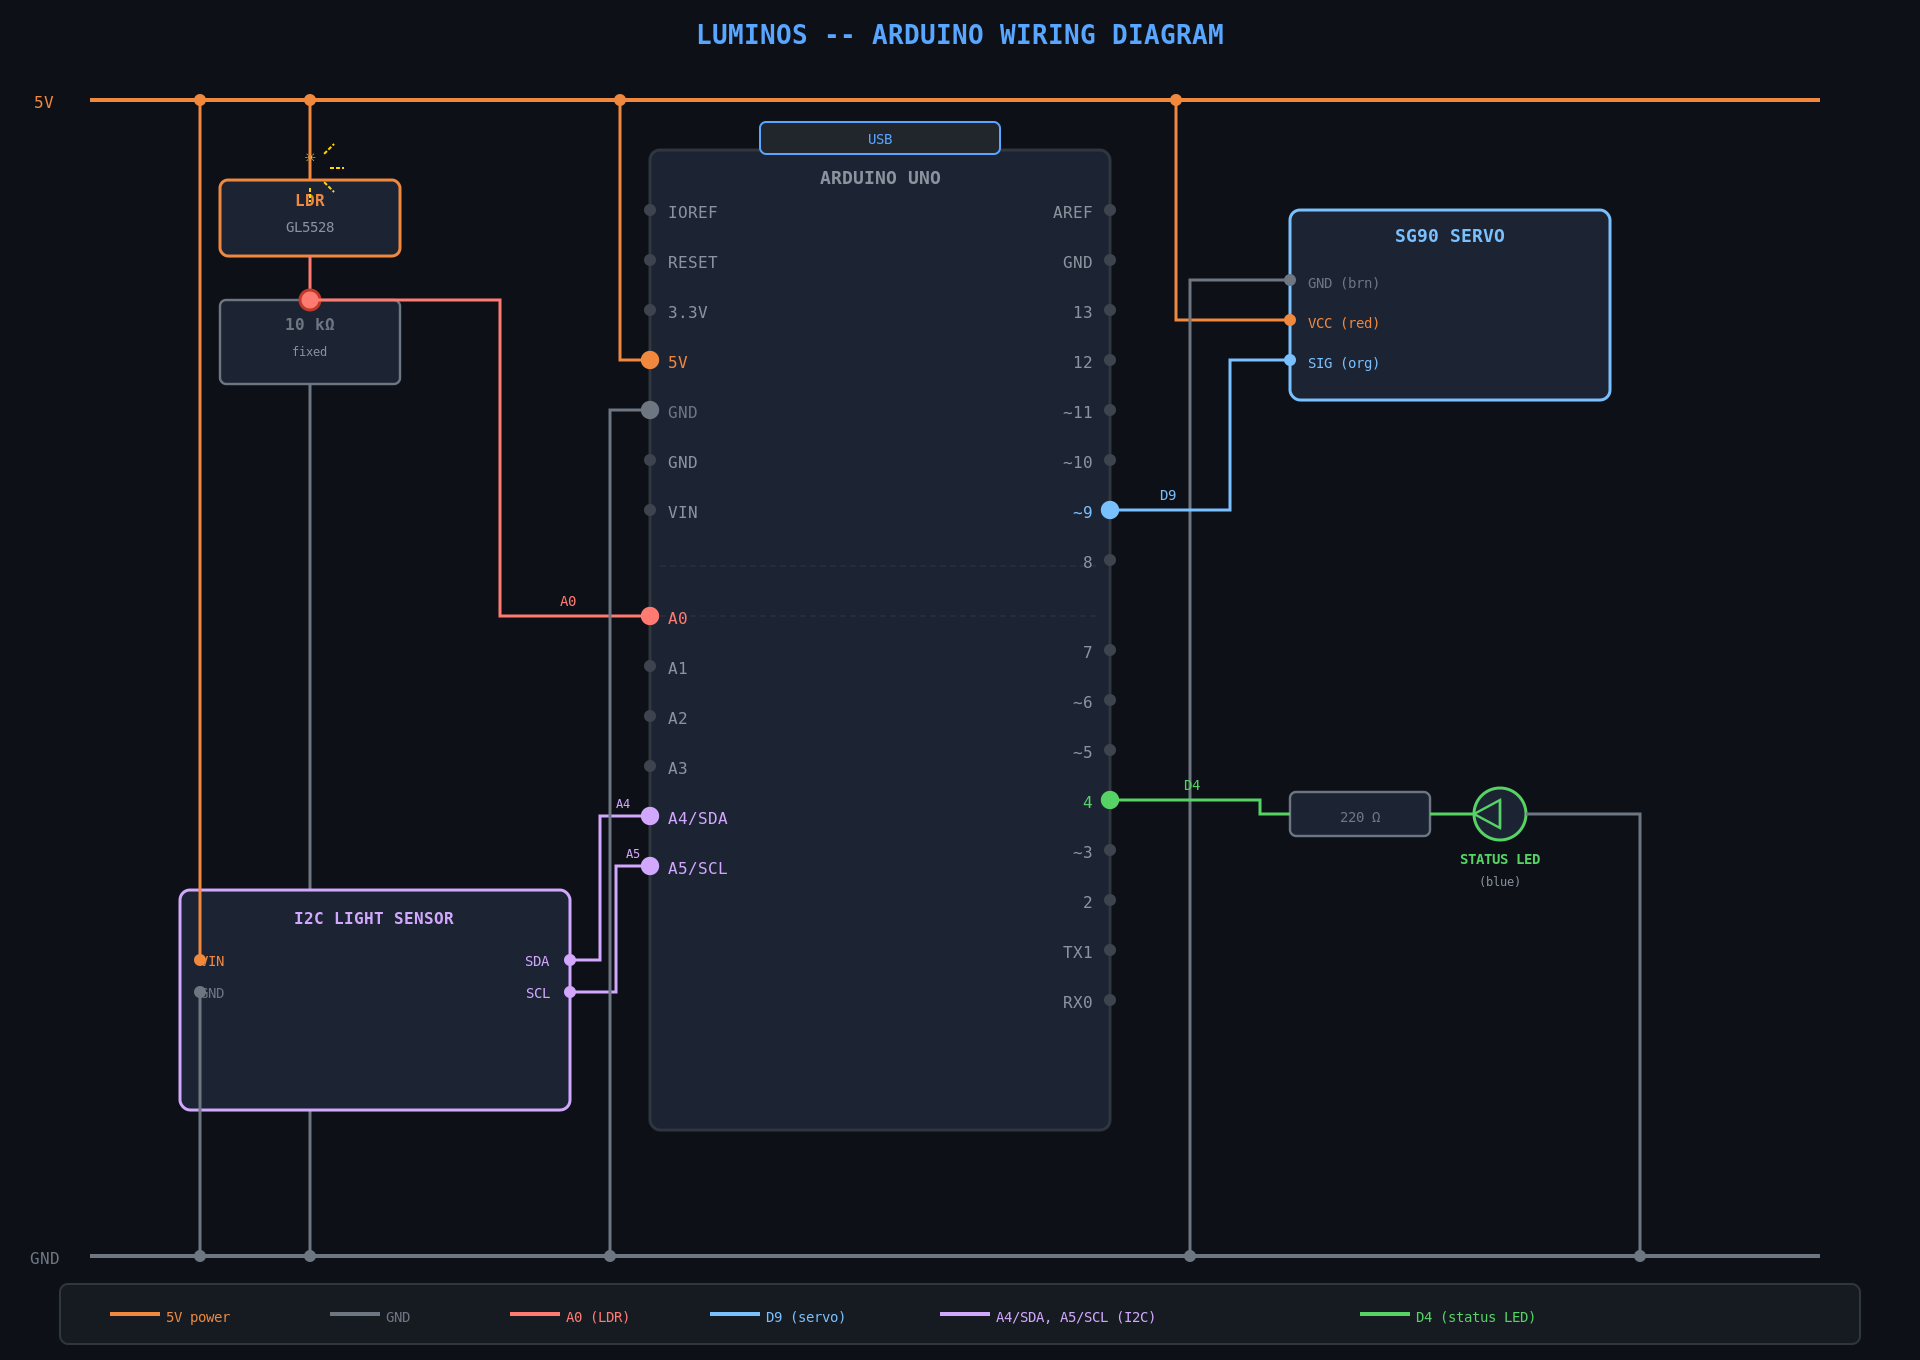
\includegraphics[width=\textwidth]{wiring_diagram.png}
  \caption{Arduino Uno wiring diagram. Left column (bottom to top): A5/SCL, A4/SDA, A3--A0, VIN, GND (x2), 5V, 3.3V, RESET, IOREF. Right column (top to bottom): AREF, GND, 13--8, 7--0. Highlighted pins are those used in this prototype.}
  \label{fig:wiring}
\end{figure}

\subsection{Active vs.\ Passive Filtration}

Three filtration approaches were considered:

\begin{enumerate}
  \item \textbf{PDLC smart film}: electrically switchable opaque/transparent.
        Rejected because small samples require 60--120~V AC and a driver circuit,
        adding cost and complexity outside the project's scope.
  \item \textbf{Electrochromic film}: voltage-variable tinting. Rejected
        because small-quantity sourcing is difficult and cost is high;
        this was already flagged as a risk in the preliminary design report.
  \item \textbf{Servo-actuated gel panel} (chosen): mechanical swing of a
        physical gel filter into the light path. Low cost, simple control
        (one PWM pin), directly observable, and maps cleanly to the three-layer
        software architecture.
\end{enumerate}

% ════════════════════════════════════════════════════════════════════════════
\section{Known Limitations and Future Work}
% ════════════════════════════════════════════════════════════════════════════

\begin{enumerate}
  \item \textbf{Absolute lux accuracy:} The GL5528 power-law model is a
        single-point calibration with a fixed $\gamma$ from the datasheet.
        A multi-point calibration against a reference lux meter would improve
        accuracy, which matters if the system is used for quantitative circadian
        dose calculations.

  \item \textbf{Bulb latency jitter:} The 0.8~s command interval was tuned for
        one specific L530 unit over one specific Wi-Fi network. On a congested
        network the latency can exceed this, leading to over-shoot. Future work
        could measure round-trip latency per command and adapt the interval
        dynamically.

  \item \textbf{Color temperature scheduling:} The current software fixes color
        temperature at 4000~K during closed-loop control. A full implementation
        would vary CCT with time-of-day as part of the circadian profile.

  \item \textbf{Multi-bulb support:} The \texttt{IP\_ADDRESS\_LIST} field
        already supports multiple IP addresses but multi-bulb simultaneous
        control has not been tested. The current architecture would serialize
        commands across bulbs, which would need to become concurrent for a
        real implementation.

  \item \textbf{Web Serial API browser support:} The current implementation
        requires Chromium-based browsers. Firefox and Safari do not support
        the Web Serial API. A fallback WebSocket bridge from a local serial
        daemon would be required for broader browser support.
\end{enumerate}

% ════════════════════════════════════════════════════════════════════════════
\section{Summary of Key Design Decisions}
% ════════════════════════════════════════════════════════════════════════════

\begin{longtable}{p{3.5cm}p{5.5cm}p{5cm}}
  \toprule
  \textbf{Decision} & \textbf{Choice Made} & \textbf{Primary Reason} \\
  \midrule
  \endfirsthead
  \multicolumn{3}{c}{\textit{(continued)}} \\
  \toprule
  \textbf{Decision} & \textbf{Choice Made} & \textbf{Primary Reason} \\
  \midrule
  \endhead
  \bottomrule
  \endlastfoot

  Lux model &
    Power-law with $\gamma=0.7$, $R_{10}=20$~k$\Omega$ &
    Matches GL5528 datasheet; single-point calibration sufficient \\
  \addlinespace

  Servo positioning &
    \texttt{writeMicroseconds()} &
    Model-independent; enables $\pm$10~$\mu$s fine nudge \\
  \addlinespace

  Servo attach/detach &
    Lazy attach, user-accessible detach command &
    Eliminates idle buzz and current draw \\
  \addlinespace

  Serial format &
    \texttt{RAW:x,VOLTAGE:x,LUX:x} &
    Human-readable; single-regex parseable \\
  \addlinespace

  Bridge threading &
    asyncio loop in daemon thread &
    Decouples slow Tapo I/O from fast HTTP handler \\
  \addlinespace

  Sensor smoothing &
    Moving average, window = 6 &
    Empirically removes ADC noise without excess lag \\
  \addlinespace

  Brightness step curve &
    Exponential clipped to [1, 5] &
    Eliminates flicker from large steps; fast convergence \\
  \addlinespace

  Reverse damping &
    3-second hold at \texttt{min\_step} on direction flip &
    Primary oscillation suppressor \\
  \addlinespace

  Command intervals &
    0.8~s normal, 2.5~s near target &
    Matched to measured bulb response latency \\
  \addlinespace

  Color temperature &
    Fixed 4000~K during auto &
    Neutral; does not interfere with lux control \\
  \addlinespace

  Serial read (React) &
    Web Serial API with TextDecoderStream &
    No server needed; browser-native; auto-reconnect \\
  \addlinespace

  Bridge polling &
    120~ms state, 70~ms sensor push &
    70~ms $>$ 25~Hz controller rate; 120~ms responsive UI \\
  \addlinespace

  Temp auto-control &
    Auto-disables when target reached &
    Convenient profile switching without permanent auto mode \\
  \addlinespace

  Alert thresholds &
    NASA SSP\_50005, 3-level &
    Consistent with ISS Human Integration Standard \\
  \addlinespace

  Filter actuation &
    Servo + Rosco gel &
    \$3--5 total; mechanically observable; no high-voltage drive \\

\end{longtable}

\end{document}
